\documentclass[10pt,aspectratio=169]{beamer}
\graphicspath{{./figures/}{./logos/}}
\usetheme[progressbar=frametitle, sectionpage=none]{metropolis}
\usepackage{appendixnumberbeamer}
\usepackage{siunitx}
\usepackage{hyperref}
\hypersetup{
colorlinks, urlcolor=blue, linkcolor={blue!10!black},
%citecolor={blue!50!black}
}
%
% metropolis theme: https://github.com/matze/mtheme
%
\mode<presentation>
{
  \usetheme{metropolis}      % or try Darmstadt, Madrid, Warsaw, ...
  %\usecolortheme{default} % or try albatross, beaver, crane, ...
  %\usefonttheme{default}  % or try serif, structurebold, ...
  \setbeamertemplate{navigation symbols}{}
  \setbeamertemplate{caption}[numbered]
} 
\definecolor{kitwaregray}{HTML}{686868}
\definecolor{kitwarelightgray}{HTML}{EEEEEE}
\definecolor{kitwareblue}{HTML}{005F9E}
\definecolor{kitwaregreen}{HTML}{009D49}
\definecolor{kitwarewhite}{HTML}{FFFFFF}
\definecolor{kitwareblack}{HTML}{000000}

\setbeamercolor{progress bar}{fg=kitwaregreen}
% Theme colors are derived from these two elements
%\setbeamercolor{alerted text}{fg=}
\setbeamercolor{frametitle}{bg=kitwareblue}
\setbeamercolor{footline}{bg=kitwaregreen}
\setbeamerfont{frame numbering}{size=\small}
\setbeamertemplate{footline}{%
  \begin{beamercolorbox}[wd=\textwidth, sep=1ex]{footline}%
    %\usebeamerfont{page number in head/foot}%
    \usebeamertemplate*{frame footer}
    \hfill%
    \usebeamertemplate*{frame numbering}
  \end{beamercolorbox}%
}
% At the logo on top of the footline.
\addtobeamertemplate{footline}{\hfill
\includegraphics[height=0.45cm]{klogo_new_crop}\hspace*{0.5em}\par}{}
%\setbeamertemplate{frame footer}{
\includegraphics[width=.1\textwidth]{klogo_new_crop}}


\title{Methods for quantitative characterization of bone injury from computer-tomography images}
%\subtitle{Methods for quantitative characterization of bone injury from computer-tomography images}
\date{\today}
\author{Pablo Hernandez-Cerdan\textsuperscript{a}, Beatriz Paniagua\textsuperscript{a}, Jack Protero\textsuperscript{b}, J.S Marron\textsuperscript{b}, Eric Libingston\textsuperscript{c}, Ted Bateman\textsuperscript{c} and Matthew McCormick\textsuperscript{a}}
\institute{\textsuperscript{a} Kitware, Inc.\newline\textsuperscript{b} Dept. of Statistics and Operations Research, UNC\newline\textsuperscript{c} Dept. of Biomedical Engineering, UNC}

\titlegraphic{
\begin{tikzpicture}[overlay, remember picture]
\node[at=(current page.south), anchor=south] {%

\includegraphics[width=.3\textwidth]{klogo}\hspace{2cm} 
\includegraphics[width=.3\textwidth]{unclogo}
};
\end{tikzpicture}
}
% \titlegraphic{\hfill\includegraphics[height=1.5cm]{logo.pdf}}

\begin{document}

\maketitle

\begin{frame}{Table of contents}
  \setbeamertemplate{section in toc}[sections numbered]
  \tableofcontents[hideallsubsections]
\end{frame}

\section{Introduction}

\begin{frame}[fragile]{Introduction}
\begin{itemize} \itemsep1em
\item Bone diseases are present in 50\% adults in the United States (CDC 2012)

\item Imaging provides a fast, scalable and non-invasive to examine bone structure. But the evaluation is often performed qualitatively or semi-quantitative.

\item Our goal is to present open source software tools to quantify musculoskeletal diseases through imaging.

\item These methods are tested on mouse femur wound model images obtained during a hemophilia study.
\end{itemize}
\end{frame}

\begin{frame}[fragile]{Materials}
\begin{itemize} \itemsep1em
\item Images acquired using microCT, with resolution of $10$\si{\micro} (\si{\micro}CT80, Scanco)
\item Trabecular bone at the proximal tibia, inferior to the growth plate
\end{itemize}
\vspace{0.5cm}
\begin{columns}[onlytextwidth]
  \column{0.5\textwidth}
    \centering
    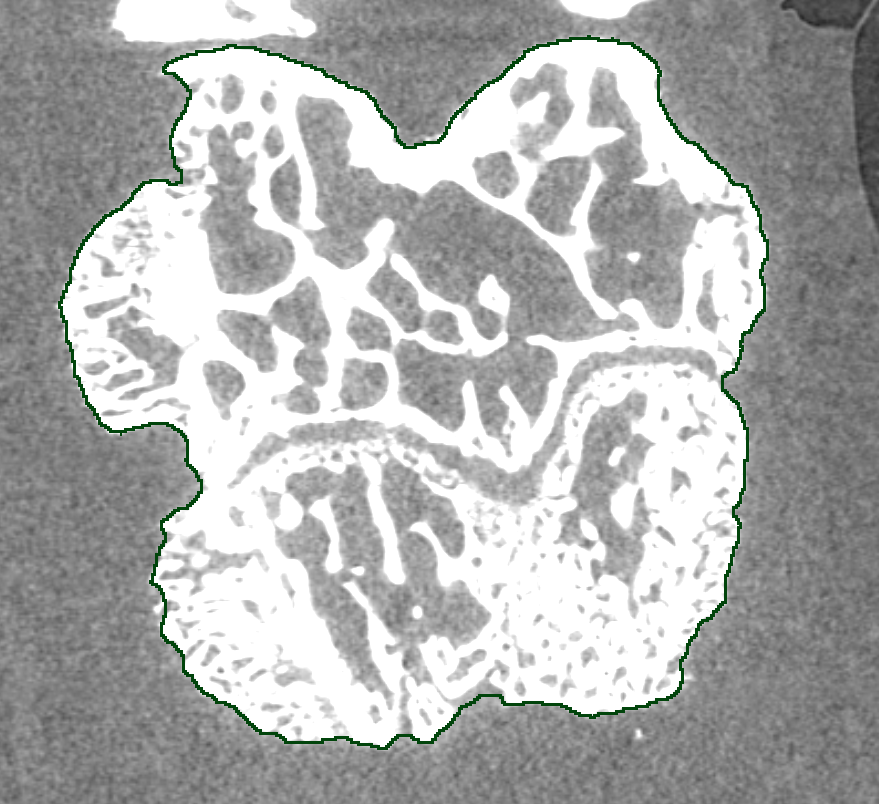
\includegraphics[width=4cm]{figures/bone_materials.png}
  \column{0.5\textwidth}
    \centering
    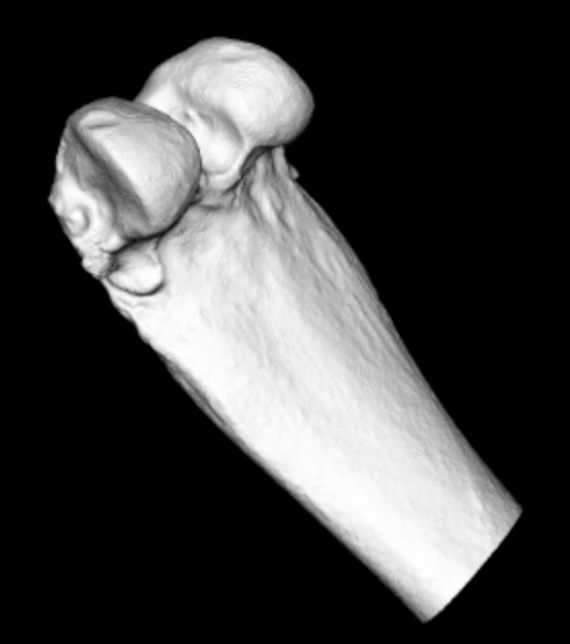
\includegraphics[width=3.7cm]{figures/bone_materials_3D.png}
\end{columns}
\end{frame}

\section{Title formats}

\begin{frame}[fragile]{Materials}
\begin{columns}[onlytextwidth]
  \column{0.25\textwidth}
    \centering
    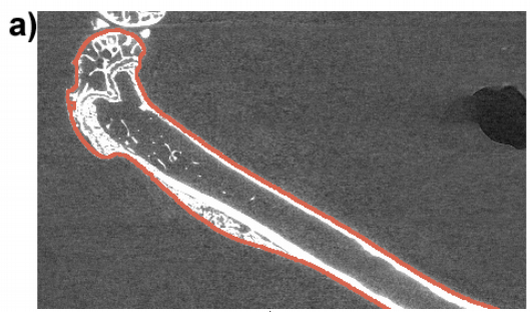
\includegraphics[width=0.99\textwidth]{figures/bone_materials_femur_highlight.png}\\
    \vspace{0.5cm}
    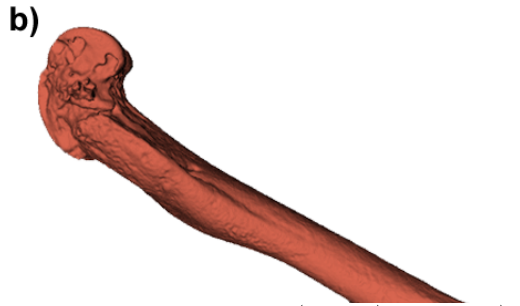
\includegraphics[width=0.99\textwidth]{figures/bone_materials_femur_3D.png}
  \column{0.75\textwidth}
    \centering
    \begin{itemize} \itemsep1em
        \item Three, 22 week old (skeletally mature), genetically modified, male mice.

        \item F8 gene knockout preventing the generation of protein coagulation factor VIII.

        \item Pathogenic pathway similar to hemophilia, presenting bleeding induced bone and joint damage.

        \item Images of right (control) and left (wounded) limbs
    \end{itemize}
\end{columns}
\end{frame}

{
\setbeamercolor{background canvas}{bg=kitwarewhite}
\begin{frame}{Image Analysis Workflow}
\begin{columns}[onlytextwidth]
    \column{0.75\textwidth}
        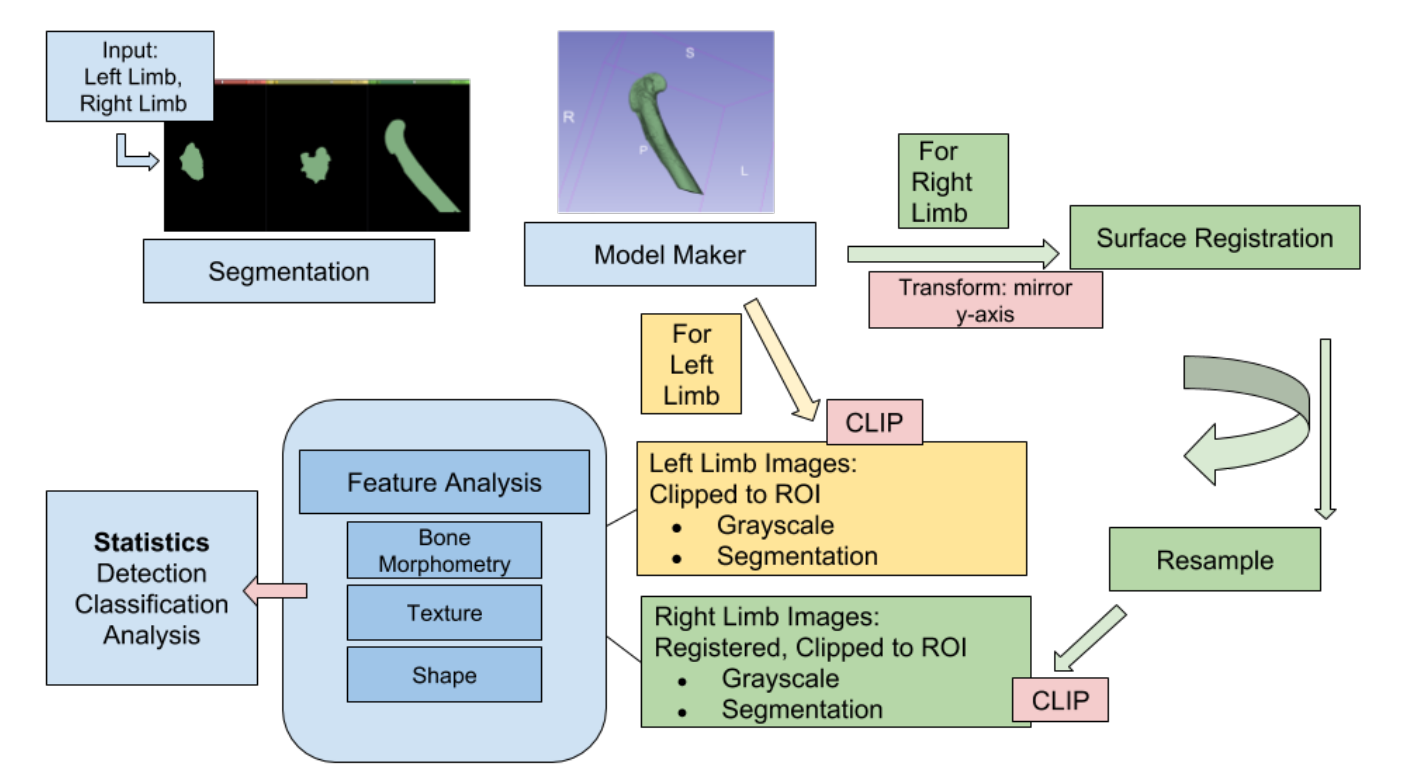
\includegraphics[width=0.99\textwidth]{figures/analysis_workflow.png}
    \column{0.25\textwidth}
        \centering
        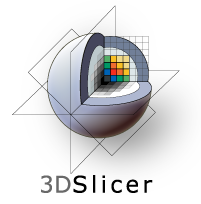
\includegraphics[width=2.5cm]{logos/logo_slicer.png}\\
        \vspace{0.3cm}
        Data and all the steps for reproducilibty at: \url{http://dx.doi.org/10.6084/m9.figshare.6947891}
\end{columns}
\end{frame}
}

\section{Elements}

\begin{frame}[fragile]{Typography}
      \begin{verbatim}The theme provides sensible defaults to
\emph{emphasize} text, \alert{accent} parts
or show \textbf{bold} results.\end{verbatim}

  \begin{center}becomes\end{center}

  The theme provides sensible defaults to \emph{emphasize} text,
  \alert{accent} parts or show \textbf{bold} results.
\end{frame}


\begin{frame}{References}
  Some references to showcase [allowframebreaks] 
\end{frame}

\section{Conclusion}

\begin{frame}{Summary}

  Get the source of this theme and the demo presentation from

  \begin{center}\url{github.com/matze/mtheme}\end{center}

  The theme \emph{itself} is licensed under a
  \href{http://creativecommons.org/licenses/by-sa/4.0/}{Creative Commons
  Attribution-ShareAlike 4.0 International License}.

\end{frame}

\begin{frame}[standout]
  Questions?
\end{frame}

\appendix

\begin{frame}[fragile]{Backup slides}
  Sometimes, it is useful to add slides at the end of your presentation to
  refer to during audience questions.

  The best way to do this is to include the \verb|appendixnumberbeamer|
  package in your preamble and call \verb|\appendix| before your backup slides.

\end{frame}

\begin{frame}[allowframebreaks]{References}

  \bibliography{references}
  \bibliographystyle{abbrv}

\end{frame}

\end{document}

